%-----------------------------------------------------------------------------80
% CONTENT
%-----------------------------------------------------------------------------80
\subsection{Entorno de desarrollo en Linux}


\begin{frame}[fragile]{Instalación de editor de código}
  \textbf{VS Code en Ubuntu y derivados}
  \begin{itemize}[<+(1)->]
   \item Descargar el paquete .deb desde \url{https://code.visualstudio.com/download}
   \item Instalar el paquete desde la terminal
    \begin{mintedbash}
      sudo dpkg -i <nombre del archivo>.deb
      sudo apt-get install -f 
    \end{mintedbash} 
   \item Actualizar el paquete e instalar code
     \begin{mintedbash}
       sudo apt-get update
       sudo apt-get install code # o también  "code-insiders"
     \end{mintedbash}
  \end{itemize}
\end{frame}

\begin{frame}[fragile]{Instalación de editor de código}
  \textbf{VS Code en Fedora/CentOS}
  \begin{itemize}[<+(1)->]
   \item Descargar el paquete .rpm desde \url{https://code.visualstudio.com/download}
   \item Instalar el paquete desde la terminal según la versión Fedora/CentOs (yum o dnf)
    \begin{mintedbash}
      yum check-update
      sudo yum install <nombre del archivo>.rpm 
    \end{mintedbash}
    \begin{mintedbash}
      dnf check-update
      sudo dnf install <nombre del archivo>.rpm 
    \end{mintedbash}
  \end{itemize}
\end{frame}

\begin{frame}[fragile]{Fortran en VS Code}
 \textbf{Fortran en VS Code}
  \begin{itemize}
   \item  En la pestaña 'Extensiones' (Ctrl+Shift+X), instalar 'fortran 2.0' encontrado con el buscador y recargar la extensión. 
  \end{itemize}
   \begin{figure}
    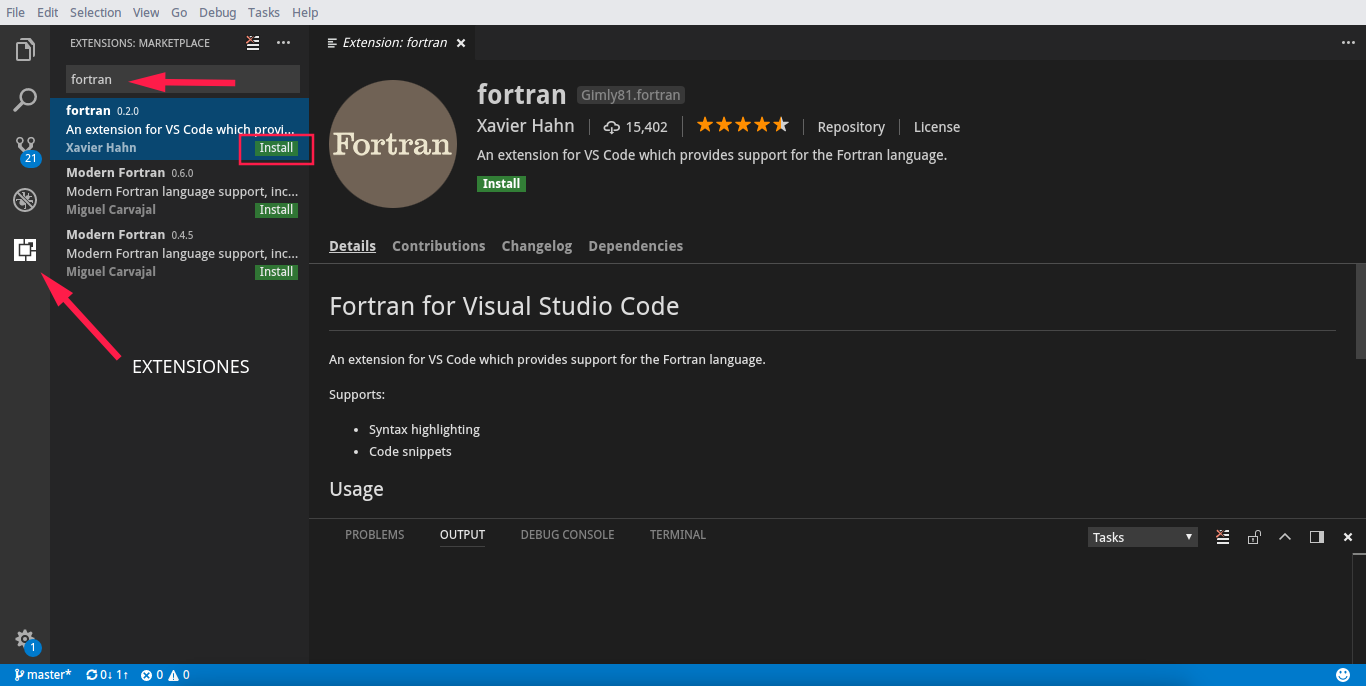
\includegraphics[width=0.95\textwidth]{./resources/vscodefortran.png}
    \caption{Extensión fortran 2.0 en VS Code}
   \end{figure}
\end{frame}

\begin{frame}[fragile]{Instalación de compilador y debuger}
  \textbf{Compilador y debugger en Ubuntu y derivados}
\begin{itemize}[<+(1)->] 
\item \textbf{Instalación de Gfortran}
    \begin{mintedbash} 
       sudo apt-get install gfortran
    \end{mintedbash}
  \item	\textbf{Instalación del paquete binutils}
    \begin{mintedbash}
       sudo apt-get update
       sudo apt-get install binutils
    \end{mintedbash}
\item	\textbf{Instalación del paquete build-essential}
    \begin{mintedbash}
       sudo apt-get update
       sudo apt-get install build-essential
  	\end{mintedbash}
\end{itemize}
\end{frame}


\begin{frame}[fragile]{Instalación de compilador y debuger}
  \textbf{Compilador y debugger en Fedora/CentOS}
\begin{itemize}[<+(1)->] 
\item	\textbf{Instalación de Gfortran}
    \begin{mintedbash}
       yum install gcc-gfortran
   	\end{mintedbash}
  \item	\textbf{Instalación del paquete Development tools}
    \begin{mintedbash}
       yum clean all
       yum groupinstall "Development tools" 
	  \end{mintedbash}
\end{itemize}
\end{frame}

